\chapter{Platform}
\label{chap:platform}

In chapter \ref{chap:intro}, I explained the motivations behind the
Custos. Chapter \ref{chap:purpose} outlines the design goals and
potential applications that these motivations suggest. In this
chapter, I'll discuss the architecture, interface, and implementation
of Custos platform.

\section{Architecture}

The Custos architecture contains several core components:

\begin{packed_item}
\item A standardized API and message exchange format promoting the
  creation and proliferation of multiple implementations across a
  selection of providers.
\item A flexible server-side authentication interface, supporting an
  extensible variety of authentication attributes.
\item A programable server-side access control system for associating
  authenticated attributes with key:value access rights on a per-key
  basis.
\item A server-side back-end key:value store for holding persistent
  user and implementation data
\item A server-side data system for storing and retrieving user data
\item A server-side auditing system for monitoring and recording
  key:value access and authentication attempt data.
\item A server-side management system for configuring and controlling
  the other components.
\item One or more client applications that offload encryption keys or
  other secrets to a Custos server for storage and access control.
\end{packed_item}

\begin{figure}[!tb]
  \vspace{5ex}
  \begin{center}
    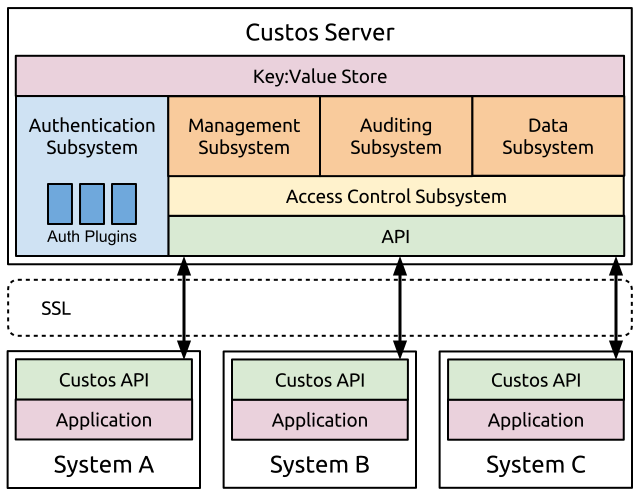
\includegraphics[width=.75\textwidth]
                    {./figs/pdf/Arch-Overview.pdf}
  \end{center}
  \caption{Basic Components of the Custos Architecture}
  \label{fig:arch-overview}
\end{figure}

Figure \ref{fig:arch-overview} shows the core Custos components. The
Custos architecture utilizes a client-server model. I'll discuss the
details of the Custos architecture in more details with respect to
both the client and server halves of the system below.

\subsection{Server}

The bulk of core Custos functionality is handled on the server
side. The server is designed to expose a single standardized API in
order to allow for a variety of inter-compatible implementations (one
possible implementation is discussed below). The Custos server
implements the following components:

\begin{packed_desc}
\item[API] \hfill \\ The server API handles all Custos requests,
  including requests for key:value data, requests to audit data
  access, and requests to modify data access controls. The API is
  essentially an RPC interface to allow applications to make requests
  of the Custos service.
\item[Access Control Subsystem] \hfill \\ The access control subsystem
  is the first step in the request processing pipeline after the
  API. The access control system compares the provided authentication
  attributes (calling into the authentication subsystem to verify
  them) to the set of required authentication attributes to determine
  if a Custos request should be allowed or denied.
\item[Authentication Subsystem] \hfill \\ The authentication
  subsystem's job is to verify the validity of any authentication
  attributes associated with a given Custos request. This subsystem is
  designed to allow for a pluggable authentication module interface
  capable of supporting a variety of authentication attributes.
\item[Data Subsystem] \hfill \\ The data subsystem is responsible for
  handling verified and accepted Custos data API requests (get, set,
  create, and delete key:value pairs). It interfaces with Key-Value
  store on one side and the access control system on the other.
\item[Auditing Subsystem] \hfill \\ The auditing subsystem is
  responsible for handling verified and accepted Custos audit API
  requests. The auditing subsystem is also concerned with logging all
  Custos requests and their corresponding responses. This data can
  then be used to generate reports related to the 'who', 'what', and
  'why' questions: \emph{Who} accessed (or failed to access)
  \emph{what} Custos stored data and \emph{why} where they granted or
  denied access (e.g. what authentication attributes did they present
  and were able to verify).
\item[Management Subsystem] \hfill \\ The management subsystem is
  responsible for handling all management related API requests after
  they have passed the authentication and access control layers. This
  primarily entails manipulating access control parameters.
\item[Key-Value Store] \hfill \\ The Key-Value store is the persistent
  data container associated with a given Custos server. It is used to
  store both end-user key:value pairs (encryption keys, etc) as well
  as a variety of internal Custos state (access control requirements,
  etc).
\end{packed_desc}

\subsection{Client}

Custos Client Application Blocks

\subsection{Authentication and Access Control}

Permissions

ACLs

Users?

\section{Interface}

\subsection{Data API Components}

For getting, setting keys

\subsection{Management API Components}

For controlling keys

\subsection{Auditing API Components}

For auditing  keys

\section{Implementation}

\subsection{API}

JSON RESTful API

\subsection{Authentication and Access Control}

Standardized module interface

\subsection{Back-end Storage}

Variable back-end key-value providers
